
\documentclass[main.tex]{subfiles}

\begin{document}

\chapter{Unloading and Reloading}
\label{LEC:unloading}

\paragraph{Outline:}
In this chapter, we introduce two concepts of inelasticity: damage and plasticity. These fundamental phenomena can be experimentally observed and distinguished upon unloading. The amount of persisting deformation shows the amount of plastic deformation (slip or strain) and the amount of stiffness reduction can be regarded as damage. These concepts allow us to model path dependent material behavior with "memory" of what loading history has it gone through so far.  
\paragraph{Addressed questions:}
\begin{itemize}
\item 
What happens in the bond structure upon unloading
\item 
Which form of inelasticity can occur?
\item 
Difference between plasticity and damage
\item 
What is hardening, what is softening?
\item 
How does the implementation of a material model for damage and plasticity work?
\end{itemize}

\section{Experimental observation}
To motivate a more general development of the model for the bond-slip behavior let us consider the case of non-monotonic loading. What happens in the material structure of the bond if the load is reduced and than it grows again? An experimental observation of the structural behavior is shown in Fig.~\ref{FIGUnloading} on an example of a double sided pullout test. The specimens had the form depicted in 
Fig.~\ref{fig:double_sided_po_test} and the embedded length was 300~mm.
This test has been conducted with textile reinforced concrete specimens reinforced with carbon fabrics. 

\begin{figure}[ht]
	\centering
  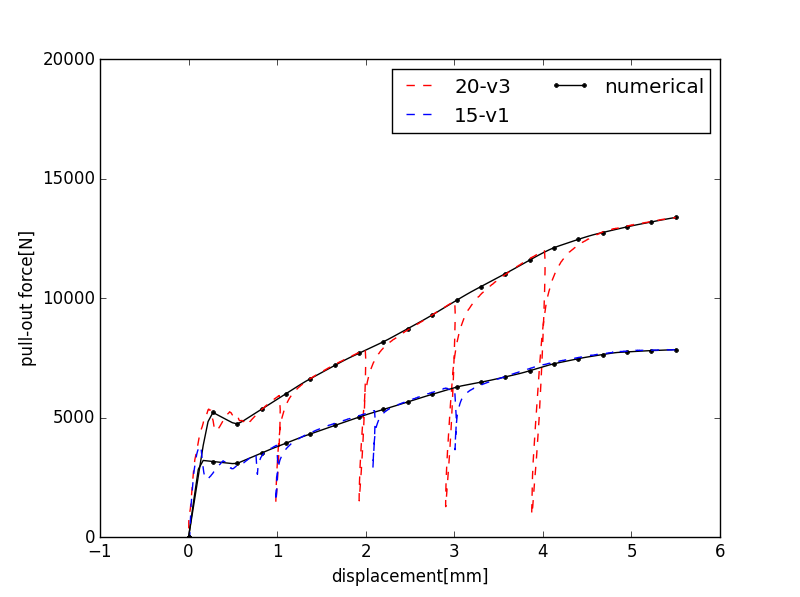
\includegraphics[width=0.7\textwidth]{fig/Lecture04/test_unloading.png}
	\caption{Double-sided pullout test with several unloading and reloading steps}
	\label{FIGUnloading}
\end{figure}

\paragraph{Question:}
Can the  pullout model from Chapter~\ref{LEC:BondBehavior} be used to desccribe such kind of behavior? Can you explain what bond stress -- slip history experienced a material point within an interface? What was the loading history leading to this test result?

The answer is, that the bond-slip models presented so far only considered monotonically increasing load and 
cannot reproduce the real material behavior upon unloading. 
The constant-bond slip model from Sec~\ref{SEC:PullOutAnalytical} and the nonlinear model using the multilinear bond-slip law exemplified in Sec~\ref{SEC:bond-slip-hardening} did not consider any change of behavior upon unloading. 
To document this statement and to show how to introduce unloading and reloading into the interactive numerical 
models  that we used in Sec~\ref{SEC:bond-slip-hardening} an example has been prepared showing how to introduce a more complex type of loading into the model.  

\begin{bmcsex}{What happens if a pullout with multilinear bond-slip law gets unloaded?}{ex41_multilinear_unloaded}
We will use the numerical examples to test the behavior interactively.
The example is provided \href{https://wiki.imb.rwth-aachen.de/do/view/IMB/Teaching/TeachExampleObj0010}{here}.
\end{bmcsex}

These solutions are limited to the monotonically increasing loading without the possibility to impose cyclic or even fatigue loading. To describe the exemplified behavior mathematically we need to introduce the irreversible phenomena of material  behavior. 
In this lecture we will first classify the types of the bond slip and establish their relation to the microscopic structure of the bond layer constituting the material behavior considering a single material point of the interface. Different types of bond material structures lead  to different types of material behavior. Cyclic loading can reveal the phenomenology of the bond we can make some conclusions about the quality of the bond: is it governed by adhesive reversible bond, or cohesive sliding or mechanical interaction between the ribs of the steel rebars and microcrack evolution within the concrete matrix?

\section{Phenomenology of the bond behavior}
\mnote{Idealization of the material structure}
Regarding a small segment of the bond interface with a nearly constant shear stress $\tau$ and constant 
slip $s$ let us try to describe the correspondence between the micro- and meso-scopic mechanisms that actually govern 
bond-slip relation $\tau(s)$. To classify the elementary mechanisms behind the observed of bond behavior, let us can idealize 
the material structure of the bond using two types of bindings:
\begin{itemize}
    \item 
as a series of elastic springs that can break once they achieve their strength 
and 
    \item
as a series of asperities representing an unevenness or roughness of the surface area. 
Sliding of these surfaces is accompanied with a stress required to cross over the asperities. 
During this process the asperities can deform elastically or get abraded.
\end{itemize}
With this simple image of the material interface we can try to associate the structure of the bond
layer with the basic types of inelastic material behavior, namely, damage and plasticity. In most cases
both types of material behavior occurr. The question is, how to distinguish them.

\mnote{Damage}
Considering the infinitesimal material point of the interface the damage type of behavior 
by a nonlinear shape of the stress-strain or (shear-slip) curve and by unloading to origin
as shown in Fig.~\ref{FIGSourcesOfDamage}. This behavior can be reproduced by a series of springs
within the considered material point representing a zone of the interface covered by elastic 
springs with scattered strength. The failure of a spring reduces the material stiffness. Since all the remaining
springs are elastic, they unload all to the origin so that after unloading, the zero slip and zero stress 
gets recovered.
\begin{figure}[ht]
	\centering
  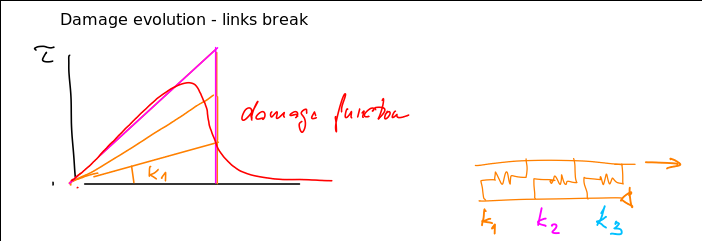
\includegraphics[width=0.7\textwidth]{drawings/damage.png}
	\caption{Bond governed by damage}
	\label{FIGSourcesOfDamage}
\end{figure}

\mnote{Plasticity}
On the other hand, if a bond stress is transfered by asperities, we can distinguish two phases of response.
Before the stress necessary to skip over an asperity has been reached, the slip is zero. At the onset of 
sliding over the asperities, the slip can increase at constant level of stress. Once the stress level 
is reduced, the slip does not change. Or putting it differently, the stress needed to induce sliding over the 
surface is constant. Once the sliding direction should be changed, 
also the sign of the shear stress must change. The described type of behavior is referred 
to as ideally plastic. This kind of material response is shown as the curve (2) in Fig.~\ref{FIGSourcesOfPlasticity}.
\begin{figure}[ht]
	\centering
  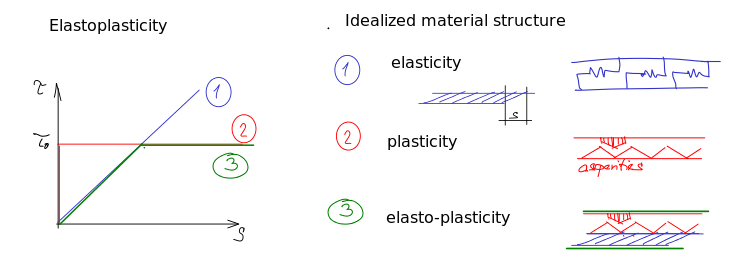
\includegraphics[width=0.7\textwidth]{drawings/plasticity.png}
	\caption{Bond governed by plasticity/friction}
	\label{FIGSourcesOfPlasticity}
\end{figure}
If asperities can deform before reaching the onset of sliding, an elastic deformation can be observed as indicated
by the curve (3) in Fig.~\ref{FIGSourcesOfPlasticity}.  
Usually, both damage and plasticity encounter simultaneously in the material behavior.
Both introduce energy dissipation. While damage is connected with the reduction of the 
material stiffness, plasticity leads to permanent deformation after unloading of the structure.
To understand the effect of damage and plasticity at the level of a material point, we will 
construct simple models that can be used within the BMCS interactive sheets to understand 
the two types of material behavior in detail.

\section{Damage model}
\label{SEC:BondDamageModel}

\mnote{stress-slip relation} 
Instead of explicitly prescribing the bond slip law as a nonlinear curve let us prescribe 
a nonlinear curve governing the evolution of stiffess.
\begin{equation}
\label{EQ:bond_damage_model}
\tau = (1 - g(\kappa))E_b \; s
\end{equation}
where $g$ is the damage function and $\kappa$ is the state variable
that depends on slip as will be explained later on. The only difference with respect to the models
used in Chapter~\ref{LEC:PullOut} is that the bond slip model introduces the 
initial bond stiffness $E_\mathrm{b}$ and prescribes its reduction in terms of the 
damage function $\omega = g{\kappa}$. The values of damage at the beginning of loading with 
intact material structure is equal to 0, and for the fully damage material it takes the value 1.
\begin{figure}[ht]
	\centering
  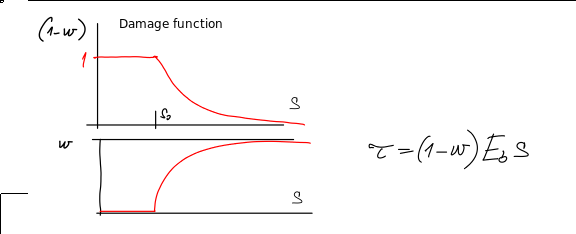
\includegraphics[width=0.7\textwidth]{drawings/damage_function.png}
	\caption{Damage function governing the deterioration process}
	\label{FIGSourcesOfDamageFunction}
\end{figure}
\mnote{effective stress}
By rearranging the terms in Eq.~(\ref{EQ:bond_damage_model}) we can introduce the notion of effective stress
as 
\begin{equation}
\tilde{\tau} = \frac{\tau}{1-\omega} = E_b \; s
\end{equation}
Apparently, this effective stress $\tilde{\tau} \geq \tau$. It can be interpreted as the stress acting on the diminishing number of springs. We can regard the damage process as the reduction of the cross-sectional area
due to the loading. The effective stress is related to the instantaneous, or still effective, cross section and not to
the initial cross sectional area of the unit material zone.

\mnote{Damage function}
By specifying the limit values of the damage function, $\omega \in (0,1)$ the question remains, 
what shape does the damage function have between these to values? The answer to this question is not unique
and depends on the particular type of material. In other words, it can only be determined using an experiment.
Let us provide two examples of the damage function that will be used later on on examples.

\subsection{Softening function [Jirasek]}
\begin{equation}
\omega = g(\kappa) = 1 - \left[\frac{s_0}{\kappa} \exp \left(- \frac{\kappa - s_0}{s_f - s_0}\right)\right]
\end{equation}
where $s_0, s_f$ are parameters controls the exponential damage function, $s_0$ is controlling the elastic limit and $s_f > s_0$ is another parameter controlling ductility.

\subsection{Softening function [Abaqus]}
The second example of the damage function taken from the finite-element program Abaqus has the form
\begin{equation}
\omega = g(\kappa) = 1 -\left(\frac{s_0}{\kappa}\right)\left[ 1 - \frac{1 - \exp(- \alpha(\frac{\kappa - s_0}{s_u - s_0})}{1 - \exp(-\alpha)}  \right]
\end{equation}
where $s_u$ is the slip at complete failure and $\alpha$ is a parameter controls the exponential damage function.

\begin{figure}[ht]
	\centering
  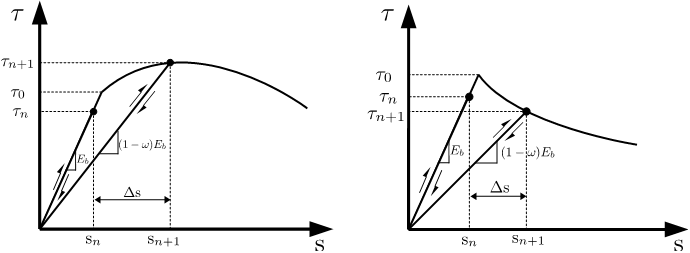
\includegraphics[scale=0.7]{fig/Damage_01.png}
	\caption{Slip - bond stress curve of damage model; left : hardening, right: softening}
	\label{FIG_damage_softening_hardening}
\end{figure}

\subsection{Hardening function [Li]}
The damage function is usually used to prescribe a material softening behavior. However, it can be adjusted rather 
flexibly to prescribe also hardening behavior. An of an analytical function is provided in the BMCS tool 
in terms of the function
\begin{equation}
\omega = g(\kappa) = \frac{\alpha_1}{1 + \exp(-\alpha_2 \kappa + 6 )}
\end{equation}
where $\alpha_1, \alpha_2$ are parameters controls the exponential damage function.

However, the exemplified damage functions do not depend directly on the slip $s$ but on a variable
$\kappa$. This variable is defined as the maximum absolute value of  slip achieved during 
the loading history, i.e.
\begin{equation}
\kappa = \mathrm{max} \{|s|\}.
\end{equation}
This parameter actually introduces the "memory" of the material point and 
introduces the different response of the material upon loading, unloading and reloading.  

The incremental time stepping used in the  numerical simulation 
is sketched in Fig.~\ref{FIG_damage_softening_hardening}. The transition between 
the linear elastic unloading response and the nonlinear growth of damage upon
increased loading is completely controlled by the state variable $\kappa$.
The damage is initiated when $\kappa > s_0$, 
where $s_0 = \tau_0 / E_b$ is the damage threshold slip. During the further simulation, 
damage can grow only if $s > \kappa$.

\begin{bmcsex}{Bond behavior governed by damage}{ex42_plastic_material_model}
\paragraph{Task:}
Study the influence of the parameters of the damage functions on the response of a single material point.
\begin{center}
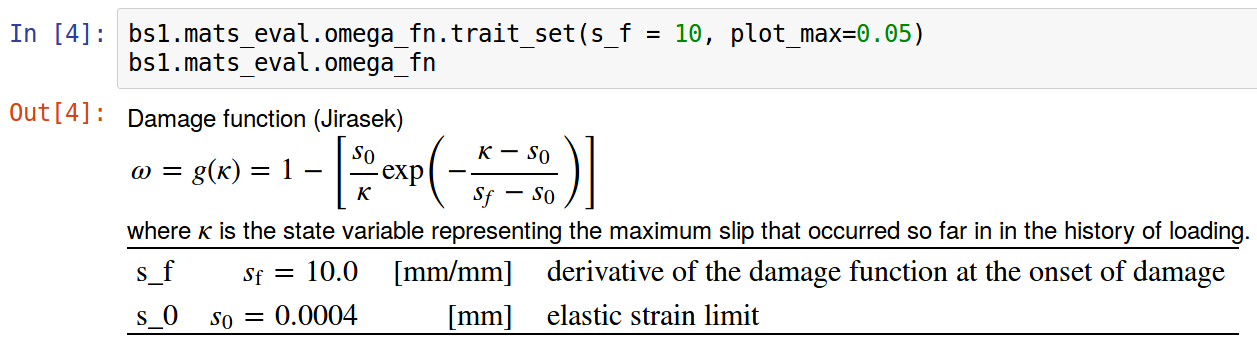
\includegraphics[width=10cm]{fig/Lecture04/damage_jirasek.png}
\end{center}
\begin{center}
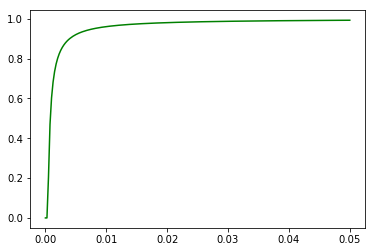
\includegraphics[width=5cm]{fig/Lecture04/damage_jirasek_function.png}
\end{center}
Use the available damage functions to reproduce both softenig and hardening behavior.
An example of a loading  scenarios and the corresponding shear-slip relation is shown below.
\begin{center}
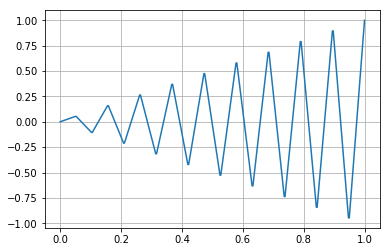
\includegraphics[width=6cm]{fig/Lecture04/damage_jirasek_loading_scenario.png}
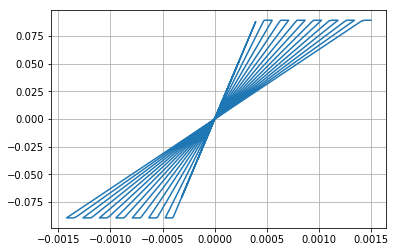
\includegraphics[width=6cm]{fig/Lecture04/damage_jirasek_stress_slip.png}
\end{center}
The other one applies slip in the range of $-\hat{s},\hat{s}$.
The interactive sheet that can be used to test this type of behavior is provided on the server.
\end{bmcsex}


%\subfile{examples/e21_bond_slip_damage/e21_bond_slip_damage}

\section{Plasticity model}
\label{SEC:BondPlasticityModel}

Considering the plastic behavior, the introduction of the material "memory" is slightly more complex.
Instead of prescribing the reduction of the material stiffness, we split 
the deformation into two variables: the elastic slip $s_\mathrm{e}$ representing the reversible
deformation, and the plastic slip $s_\mathrm{p}$ expressing the irreversible deformation 
that would persist after unloading. Let us note, that the development of the plastic slip 
$s_\mathrm{p}$ depends on the loading history. As a consequence, the variable $s_\mathrm{p}$ 
introduces a kind of material "memory" that remembers the loading events and their levels that 
the material point experienced so far. This variable plays a similar role as the 
variable $\kappa$ introduced for the damage model in Sec.~\ref{SEC:BondDamageModel}

The total slip is defined as
\begin{align}
s = s_\mathrm{e} + s_\mathrm{p}.
\end{align}
We can start to construct the bond-slip behavior by expressing the elastic behavior of the material 
$\tau = E_\mathrm{b} s_\mathrm{e}$ as 
\begin{equation}
\tau = E_\mathrm{b} (s - s_\mathrm{p}).
\end{equation}
where $\tau$ is the bond stress, $E_\mathrm{b}$ is the bond stiffness and $s, s_\mathrm{p}$ are the total slip and the plastic slip respectively. 
As a next step, we require that the bond stress yields once it achieves the prescribed level. 
This is done in terms of an inequality 
\begin{equation}
\label{eq:yield_limit}
f = |\tau - X| - h \leq 0
\end{equation}
imposing a yield limit on the value of shear stress  $\tau$. This function defines the elastic range of the 
material response. Once this limit is reached, an inelastic yielding occurs. 
The symbols $h$ and $X$ introduce two different types of limit of the bond stress.

The variable $h$ represents the so called isotropic limit relative to the zero stress. In other words,
the limit stress is the same for the negative and positive stresses. It is defined as
\begin{equation}
h = \mathrm{max}\{0 , (K z + \tau_0)\}
\end{equation}
where $K$ is the isotropic hardening parameter, $\tau_0$ is the yield stress. $z$ represents the state 
variable of a material point. It is a part of the "memory" in addition to plastic slip $s_\mathrm{p}$. 

The variable $X$ represents the kinematic limit. It is relative to the level of stress achieved during 
the history. A linear kinematic 
hardening behavior is defined as 
\begin{equation}
X = \gamma \; \alpha
\end{equation}
where $\gamma$ is kinematic hardening parameter and $\alpha$ is the kinematic hardening state variable
that "memorizes" the effect of the  loading history.

By defining the threshold or yield limit we specify the range of elastic behavior. As a next step we need to tell what happens once this limit has been reached and the loading still increases. 
The usual way to define the response in an inelastic regime is to introduce the flow rule 
governing the plastic deformation, i.e. plastic slip, as the 
derivative of the yield limit with respect to the stress $\tau$
\begin{equation}
\label{eq:s_p}
\dot{s}^p = \dot{\lambda} \; \frac{\partial f}{\partial \tau} = \dot{\lambda} \; \mathrm{sign}(\tau - X).
\end{equation}
where $\dot{\lambda}$ is an unknown scalar multiplier. In this way, we have defined the direction of flow
but not its magnitude that is represented by $\dot{\lambda}$.
The flow rules for the remaining state variables $z$ and $\alpha$ 
are defined in the same way, i.e. by differentiating the yield limit with respect to the corresponding (conjugate) 
stress, i.e. $h$ and $X$
\begin{align}
\label{eq:isotropic_hardening}
& \mathrm{\mbox{Isotropic hardening}} \qquad \dot{z} = \dot{\lambda}\\
\label{eq:kinematic_hardening}
& \mathrm{\mbox{Kinematic hardening}} \qquad \dot{\alpha} = \dot{\lambda} \; \mathrm{sign}(\tau - X).
\end{align}
Having expressed the evolution of the state variables in terms of a single scalar parameter $\dot{\lambda}$
we need to find another criterion to get its value. This criterion is derived from the fact, that upon loading beyond the elastic limit, the state of a material point must stay on the yield surface. The only way how this can be accomplished is that the yield surface changes during the yielding process. Let the change of the yield limit is expressed as $\dot{f}$, representing the derivative with respect to a control parameter of the loading.

Then, two conditions can be imposed in  an inelastic regime. 
\begin{itemize}
    \item
The first is the  requirement that the the stress state does not exceed the yield limit, i.e.
\begin{equation}
\dot{\lambda} \geq 0, \hspace{50pt}  f\leq 0, \hspace{50pt} \dot{\lambda} f = 0
\end{equation}
This form is the so called Kuhn-Tucker condition (loading-unloading condition).
It says that the plastic multiplier $\dot{\lambda}$ must be zero in elastic regime and it grow only if the yield limit has been reached. 
\item
Second, we require that the derivative of the yield limit stays also zero
\begin{equation}
\label{eq:consistency_condition}
\dot{\lambda} \geq 0, \implies   f = 0, \longrightarrow  \dot{f} = 0
\end{equation}
which means that the inelastic variables can only grow if the stress stays on the yield limit. Thus, during the yielding, the yield limit can grow or shrink. 

This fact is closely related to the phenomena of hardening and softening discussed in theprevious lectures. Closer look at the considered yield limit given in (\ref{eq:yield_limit}) reveals that the material parameters $K$ and $\gamma$ define the rate of expansion or shrinkage of the  elastic domain. Negative values of $K$ and $\gamma$ introduce a linear softening behavior. The condition (\ref{eq:yield_limit}) represents the equation that delivers the value of the plastic multiplier $\dot{\lambda}$ to deliver the amount of yielding corresponding to the current load.
\end{itemize}


\begin{bmcsex}{Bond behavior governed by plasticity}{ex43_plastic_material_model}
The example presents a plastic material model with isotropic and kinematic hardening.
Two loading scenarios are shown, one for increasing amplitude and unloading to zero slip.
\begin{center}
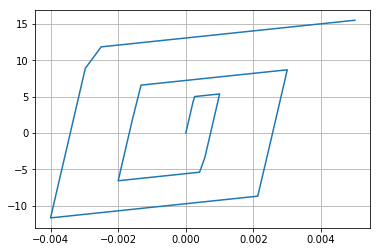
\includegraphics[width=6cm]{fig/Lecture04/ep_stress_slip.png}
\end{center}
The other one applies slip in the range of $-\hat{s},\hat{s}$.
The interactive sheet that can be used to test this type of behavior is provided on the server
\end{bmcsex}

Thus, to solve for $\dot{\lambda}$ the derivative of the yield surface needs to be expressed using the previously introduced equations
\begin{align}
\dot{f} &= \frac{\partial f}{\partial \tau} \dot{\tau} +
\frac{\partial f}{\partial z} 
\dot{z} +
\frac{\partial f}{\partial \alpha} \dot{\alpha}
\nonumber \\
&= \frac{\partial f}{\partial \tau} E_\mathrm{b} ( \dot{s} - \dot{s}_\mathrm{p} )
+ \ldots \mathrm{complete}
\nonumber \\
&= \mathrm{sign}(\tau - X) E_\mathrm{b} (( \dot{s} - \dot{s}_\mathrm{p} )
+ \ldots \mathrm{complete}
\nonumber \\
&= \mathrm{sign}(\tau - X) E_\mathrm{b} ( \dot{s} - \dot{\lambda} \, \mathrm{sign}(\tau - X)  )
+ \ldots \mathrm{complete}
\nonumber \\
&= \mathrm{sign}(\tau - X) \, E_\mathrm{b}
\, \dot{s} 
- 
\mathrm{sign}(\tau - X) \mathrm{sign}(\tau - X) \,
E_\mathrm{b}
\dot{\lambda} 
+ \ldots \mathrm{complete}
\nonumber \\
&= \mathrm{sign}(\tau - X) \, E_\mathrm{b}
\, \dot{s} 
- 
E_\mathrm{b}
\dot{\lambda}
+ \ldots \mathrm{complete}
\nonumber \\
&= 0
\end{align}
As a result the plastic multiplier for the current step can be expressed as 
\begin{align}
\dot{\lambda} = \mathrm{sign}(\tau - X) \, \dot{s} 
+ \ldots \mathrm{complete}
\end{align}
The resolved multiplier can than be substituted back into the evolution equations (\ref{eq:s_p}), (\ref{eq:isotropic_hardening}) and (\ref{eq:kinematic_hardening}) to obtain the explicit first-order differential equations 
\begin{align}
\dot{s}^p &= 
\mathrm{sign}(\tau - X) 
\mathrm{sign}(\tau - X) 
\, \dot{s}
= \dot{s}
\\ 
\dot{z} 
&= \mathrm{sign}(\tau - X) \dot{s}
\\
\dot{\alpha} &= 
\mathrm{sign}(\tau - X)  \mathrm{sign}(\tau - X) \, \dot{s}
= \dot{s}
\end{align}
Note that isotropic hardening grows regardless of the sign of the total slip rate. It's sign gets canceled by the term $\mathrm{sign}(\tau - X)$ which is the same as the of $\dot{s}$. On the other hand, the plastic slip and kinematic hardening grow consistently with the direction of the total (control) slip.

The described derivation delivers the differential evolution equations that are continuous. To solve them for a particular problem at hand, an integration scheme to derive a time-stepping algorithm must be applied. The standard procedure applied in the nonlinear material models for finite-element simulations applies the return mapping algorithm sketched in the next section. 

\section{Return mapping algorithm}

The algorithmic treatment of plasticity requires the incremental formulation 
of the evolution equations. To provide a robust implementation, 
we need to make the distinction between an elastic and plastic state of the material.
If the material is a plastic state, than the consistency condition is used
to return back to the yield limit as shown in Fig.~\ref{FIGReturnMapping2}.

\begin{figure}[ht]
	\centering
  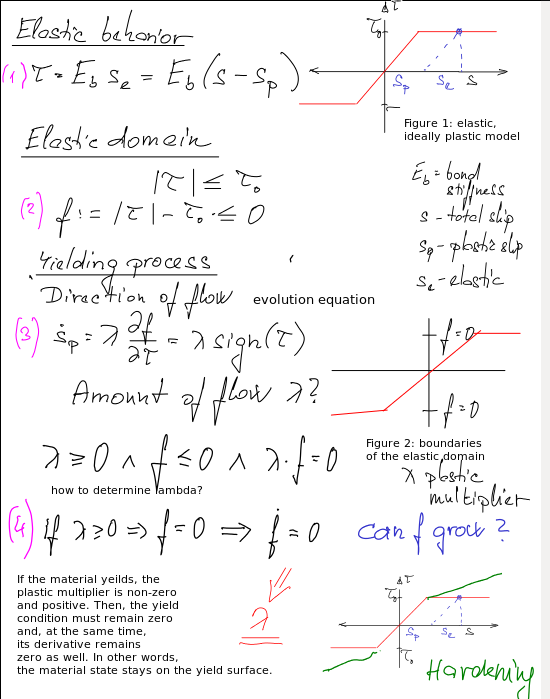
\includegraphics[width=7.5cm]{drawings/plasticity_how_much_yielding.png}
  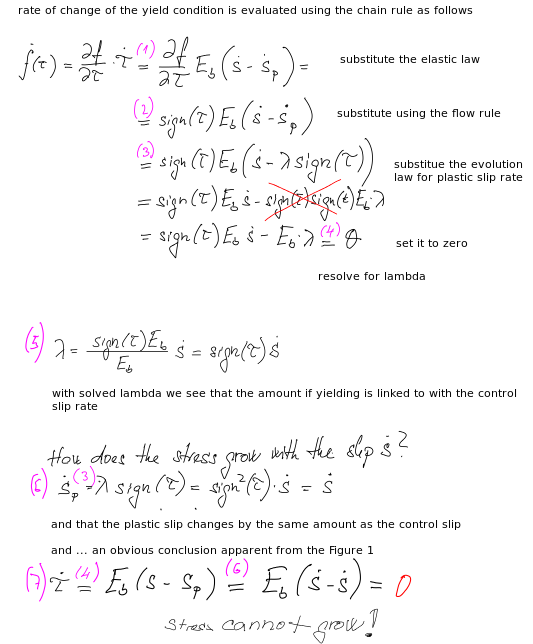
\includegraphics[width=7.5cm]{drawings/plasticity_how_much_yielding2.png}
	\caption{What happens beyond elastic domain? Example of elastic-ideally plastic bond.}
	\label{FIGReturnMapping1}
\end{figure}


input date : $s_n,\Delta_s , \tau_n , s^p_n, \alpha_n , z_n$\\
output date : $ \tau_{n+1} , s^p_{n+1}, \alpha_{n+1} , z_{n+1}$\\
constant material parameters: $E_b, \tau_0, K, \gamma $
\begin{figure}[t]
	\centering
  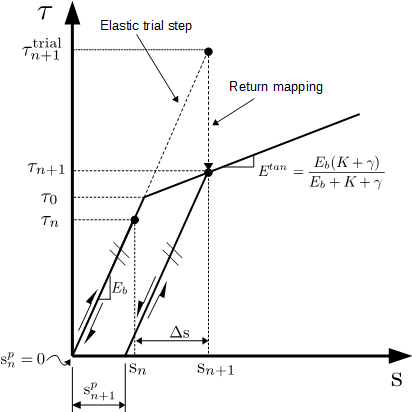
\includegraphics[scale=0.6]{fig/PLasticity_return_mapping.png}
	\caption{Return mapping of the plasticity model}
	\label{FIGReturnMapping2}
\end{figure}
\begin{align*}
&s_{n+1} = s_n + \Delta_s \\
&\tau^{trial}_{n+1} = E_b (s_{n+1} - s^p_n)\\
&X_{n} = \gamma \alpha_n \\
&h = \mathrm{max}\{0 , (K z_n + \tau_0)\}\\
&f^{trial}_{n+1} = |\tau^{trial}_{n+1} - X_{n}| - h
\end{align*}
If $f^{trial}_{n+1} \leq 0$ $\longrightarrow$ Elastic step
\begin{align*}
&\tau_{n+1} = \tau^{trial}_{n+1}\\
&(.)_{n+1} = (.)_{n}
\end{align*}
with $(.)$ denote the state variables $(s^p, \alpha, z)$\\\\
Else $\longrightarrow$ Plastic step: perform return mapping
\begin{align*}
&\Delta \lambda = \frac{f^{trial}_{n+1}}{E_b + |K| + \gamma}\\
&s^p_{n+1} = s^p_{n} + \Delta \lambda \; \mathrm{sign}(\tau^{trial}_{n+1} - X_n)\\
&z_{n+1} = z_n + \Delta \lambda \\
&\alpha_{n+1} = \alpha_{n} + \Delta \lambda \;  \mathrm{sign}(\tau^{trial}_{n+1} - X_n)\\
& \tau_{n+1} = \tau^{trial}_{n+1} - E_b \Delta \lambda \; \mathrm{sign}(\tau^{trial}_{n+1} - X_{n})
\end{align*}

%\subfile{examples/e22_bond_slip_plasticity_kinem/e22_bond_slip_plasticity_kinem}

\section{Damage-Plasticity model}

This section summarizes the contents of the two previous sections within a single model
covering both damage and plasticity. Such type of models is implemented in the nonlinear
finite element packages and is used for the simulation of concrete behavior.
\begin{description}
  \item[$\bullet$ Stress-slip relation] 
\end{description}
\begin{equation}
\tau = (1 - \omega)E_b (s - s^p)
\end{equation}
where $\omega$ is the damage parameter

\begin{description}
  \item[$\bullet$ The effective stress] 
\end{description}
\begin{equation}
\tilde{\tau} = \frac{\tau}{1-\omega} = E_b (s - s^p)
\end{equation}

\begin{description}
  \item[$\bullet$ Plastic yield function] 
\end{description}
\begin{equation}
f = |\tilde{\tau} - X| - h
\end{equation}
where
\begin{equation}
h = \mathrm{max}\{0 , (K z + \tau_0)\}
\end{equation}

\begin{description}
  \item[$\bullet$ Damage function] 
\end{description}
for example using the following damage function:
\begin{equation}
\omega = g(\kappa) = \frac{\alpha_1}{1 + \exp(-\alpha_2 \kappa + 6 )}
\end{equation}
where $\alpha_1, \alpha_2$ are parameters control the exponential damage function, and $\kappa$ is the history parameter which defines the maximum absolute value of the slip during the loading history and can be written as follows
\begin{equation}
\kappa = \mathrm{max} \{|s|\}
\end{equation}
\begin{description}
  \item[$\bullet$ Damage thershold] 
\end{description}
The damage is active when $\kappa > s_0$, 
where $s_0 = \tau_0 / E_b$ is the damage threshold slip

\begin{description}
  \item[$\bullet$ Flow rule ] 
\end{description}
\begin{equation}
\dot{s}^p = \dot{\lambda} \; \mathrm{sign}(\tilde{\tau} - X)
\end{equation}
where $\dot{\lambda}$ is the incremental multiplier.
\begin{description}
  \item[$\bullet$ Hardening rules] 
\end{description}
\begin{align}
& \mathrm{\mbox{Isotropic hardening}} \qquad \dot{z} = \dot{\lambda}\\
& \mathrm{\mbox{Kinematic hardening}} \qquad \dot{\alpha} = \dot{\lambda} \; \mathrm{sign}(\tilde{\tau} - X)
\end{align}\\ 
with 
\begin{equation}
X = \gamma \; \alpha
\end{equation}
where $\gamma$ is kinematic hardening parameter.

\begin{description}
  \item[$\bullet$ Kuhn-Tucker condition (loading-unloading condition)] 
\end{description}
\begin{equation}
\dot{\lambda} \geq 0, \hspace{50pt}  f\leq 0, \hspace{50pt} \dot{\lambda} f = 0
\end{equation}

\begin{description}
  \item[$\bullet$ Consistency condition)] 
\end{description}
\begin{equation}
\dot{\lambda} \geq 0, \longrightarrow  f = 0, \longrightarrow  \dot{f} = 0
\end{equation}

\begin{description}
  \item[$\bullet$ Return mapping algorithm]
\end{description}
input date : $s_n,\Delta_s , \tau_n , \omega_n ,\kappa_n , s^p_n, \alpha_n , z_n$\\
output date : $ \tau_{n+1} , \omega_{n+1}, \kappa_{n+1}, s^p_{n+1}, \alpha_{n+1} , z_{n+1}$\\
constant material parameters: $E_b, \tau_0, K, \gamma , \beta , s_0 ,s_f $
\begin{align*}
&s_{n+1} = s_n + \Delta_s
\end{align*}

\begin{description}
  \item[Damage] 
\end{description}
If $s_{n+1} \leq s_0$ $\longrightarrow$ No damage \\
\begin{align*}
&\omega_{n+1} = 0 
\end{align*}
Else $\longrightarrow$ Damage is active \\
\begin{align*}
& \kappa_{n+1} = \mathrm{max}(|s_{n+1}|, \kappa_n)\\
& \omega_{n+1} = g(\kappa) = \frac{\alpha_1}{1 + \exp(-\alpha_2 \kappa_{n+1} + 6 )}
\end{align*}

\begin{description}
  \item[Plasticity] 
\end{description}

\begin{align*}
&\tilde{\tau}^{trial}_{n+1} = E_b (s_{n+1} - s^p_n)\\
&X_{n} = \gamma \alpha_n \\
&h = \mathrm{max}\{0 , (K z_n + \tau_0)\}\\
&f^{trial}_{n+1} = |\tilde{\tau}^{trial}_{n+1} - X_{n}| - h
\end{align*}
If $f^{trial}_{n+1} \leq 0$ $\longrightarrow$ Elastic step
\begin{align*}
&\tilde{\tau}_{n+1} = \tilde{\tau}^{trial}_{n+1}\\
&\tau_{n+1} = (1- \omega_{n+1}) \tilde{\tau}_{n+1} \\
&(.)_{n+1} = (.)_{n}
\end{align*}
with $(.)$ denote the state variables $(s^p, \alpha, z)$\\\\
Else $\longrightarrow$ Plastic step: perform return mapping
\begin{align*}
&\Delta \lambda = \frac{f^{trial}_{n+1}}{E_b + |K| + \gamma}\\
&s^p_{n+1} = s^p_{n} + \Delta \lambda \; \mathrm{sign}(\tau^{trial}_{n+1} - X_n)\\
&z_{n+1} = z_n + \Delta \lambda \\
&\alpha_{n+1} = \alpha_{n} + \Delta \lambda \;   \mathrm{sign}(\tau^{trial}_{n+1} - X_n)\\
& \tau_{n+1} = (1- \omega_{n+1}) E_b (s_{n+1} - s^p_{n+1})
\end{align*}

%\subfile{examples/e23_bond_slip_damage_plasticity/e23_bond_slip_damage_plasticity}

\end{document}